\documentclass[a4paper]{article}

\usepackage{amsmath,amsfonts,amsthm,amssymb,mathtools} % Math packages
\usepackage[utf8]{inputenc} % Required for non-English characters
\usepackage[english]{babel} % Spell-checking
\usepackage{fancyhdr} % Required for custom headers
\usepackage{lastpage} % Required to determine the last page for the footer
\usepackage{extramarks} % Required for header and footer marks
\usepackage[margin=1.2in]{geometry} % Sets page margin
\usepackage{esdiff} % Defines commands for differentials
\mathtoolsset{showonlyrefs} % Only referenced equations are numbered
\usepackage{xfrac} % Allows for slanted fractions using \sfrac{*}{*}
\usepackage{graphicx} % For pictures
\usepackage{physics}
\usepackage{bm}

% The following sets up the header and footer
\fancyhf{}
\pagestyle{fancy}
\lhead{\hmwkCourse} %left header
\rhead{\hmwkTitle \, \textendash \, \hmwkName \, \textendash \, \hmwkClass} % right header
\rfoot{Page\ \thepage\ of\ \pageref{LastPage}} % right footer
\renewcommand\headrulewidth{0.4pt} % Size of the header rule
\renewcommand\footrulewidth{0.4pt} % Size of the footer rule

% The following sets the information shown in header and footer
\newcommand{\hmwkTitle}{Homework 2} % Assignment title
\newcommand{\hmwkCourse}{Optics} % Course/class
\newcommand{\hmwkName}{John Meneghini} % Your name
\newcommand{\hmwkClass}{2/9/2024}

% The following sets new paragraphs to start with a line skip instead of an indentation. Just my preference.
\setlength{\parindent}{0pt} %No indentation of new paragraphs
\setlength{\parskip}{10pt}

\begin{document}

\section*{Question 1}
Two thin lenses having focal lengths of $+15.0 cm$ and $-15.0$ cm respectively are positioned $60.0$ cm
apart. A page of print is held $25.0$ cm in front of the positive lens. Describe, in detail, the image of the
print (i.e. insofar as it’s paraxial). \\\\

\begin{center}
    $s_1 = 25.0$ cm, $f_1 = 15.0$ cm, $f_2 = -15.0$ cm, and $d = 60.0$ cm.
\end{center}
$$ \frac{1}{f_1} = \frac{1}{s_1} + \frac{1}{p_1} \rightarrow  \frac{1}{p_1} = \frac{1}{15.0} - \frac{1}{25.0}$$
$$ p_1 = 37.5 \textrm{ cm}$$
$$ \frac{1}{f_2} = \frac{1}{d - p_1} + \frac{1}{p_2} \rightarrow  \frac{1}{p_2} = -\frac{1}{15.0} - \frac{1}{60 - 37.5}$$
$$ p_2 = -9.0 \textrm{ cm}$$\\
What about magnification?
$$ m = m_1 m_2 = \left( - \frac{p_1}{s_1}\right) \left( - \frac{p_2}{s_2}\right)$$
$$ m = \left(-\frac{37.5}{25.0}\right) \left(\frac{9}{60-37.5}\right) = -0.5984$$
So, the image will be virtual, 9.0 cm in front of the negative lens (between the lenses), 0.5984 times smaller, and inverted.

\newpage
\section*{Question 2}
Draw a ray diagram for the combination of two positive lenses wherein their separation equals the
sum of their respective focal lengths. Do this carefully, with a ruler. You may do your sketch on the
arrangement shown on the last page of this assignment

\begin{figure*}[htb!]
    \centering
    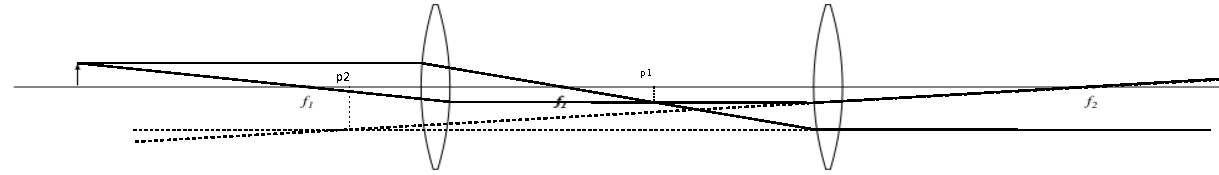
\includegraphics[angle=90]{hw2q2.pdf}
\end{figure*}

\section*{Question 3}
Consider the case of two positive thin lenses, $L_1$ and $L_2$, separated by 5 cm. Their diameters are
6 cm and 4 cm, respectively, and their focal lengths are $f_1 = 9$ cm and $f_2 = 3$ cm. If a diaphragm with a
hole 1 cm in diameter is located between them, 2 cm from $L_2$, find the aperture stop and the locations
and sizes of the pupils for an axial point, $S$, 12 cm in front of (to the left of) $L_1$.\\\\

In order to determine the aperture stop, we can trace a separate ray from the axial point to the margin of each potential aperture stop. We then can back out the initial angle of the rays, and which potential stop resulted in a smaller angle will be the aperture stop. This will determine angle of the marginal ray.

Lets call the initial ray at the axial point $S$, $\va{r}_S = \begin{bmatrix}
    0 \\
    \alpha_0
\end{bmatrix} $, where $\alpha_0$ is the initial angle we're trying to determine. The translation matrix that will bring $\va{r}_S$ to $L_1$ is

$$ \bm{T_1} = \begin{bmatrix}
    1 & 12 \\
    0 & 1 \\
\end{bmatrix} $$
and we want to find the $\alpha_0$ which satisfies the following matrix equation

$$ \begin{bmatrix}
    1 & 12 \\
    0 & 1 \\
\end{bmatrix}
\begin{bmatrix}
    0 \\
    \alpha_0
\end{bmatrix} =
\begin{bmatrix}
    3 \\
    \alpha_0
\end{bmatrix} $$

Solve this matrix equation gives

$$ \alpha_0 = 0.25 $$

Now for the diaphragm, the matrix that will bring $\va{r}_S$ to the margin of the diaphragm is given by the following matrix

$$ \bm{T_d}\bm{R_1}\bm{T_1} = \begin{bmatrix}
    1 & 3 \\
    0 & 1 \\
\end{bmatrix}
\begin{bmatrix}
    1 & 0 \\
    -\frac{1}{9} & 1 \\
\end{bmatrix}
\begin{bmatrix}
    1 & 12 \\
    0 & 1 \\
\end{bmatrix} = 
\begin{bmatrix}
    \frac{2}{3} & 11\\
    - \frac{1}{9} & - \frac{1}{3}
\end{bmatrix}$$

So, the matrix equation is 

$$ \begin{bmatrix}
    \frac{2}{3} & 11\\
    - \frac{1}{9} & - \frac{1}{3}
\end{bmatrix}
\begin{bmatrix}
    0 \\
    \alpha_0
\end{bmatrix}
=
\begin{bmatrix}
    \frac{1}{2}   \\
    \alpha_{new}
\end{bmatrix}$$

Solving,
$$\alpha_{0} = 0.045$$

Next, find the matrix that will bring $\va{r}_S$ to the margin of the second lens

$$ \bm{T_2}\bm{T_d}\bm{R_1}\bm{T_1} = 
\begin{bmatrix}
    1 & 2\\
    0 & 1
\end{bmatrix}
\begin{bmatrix}
    \frac{2}{3} & 11\\
    - \frac{1}{9} & - \frac{1}{3}
\end{bmatrix} =
\begin{bmatrix}
    \frac{4}{9} & \frac{31}{3}\\
    - \frac{1}{9} & - \frac{1}{3}
\end{bmatrix}
$$

Then, our matrix equation is
$$
\begin{bmatrix}
    \frac{4}{9} & \frac{31}{3}\\
    - \frac{1}{9} & - \frac{1}{3}
\end{bmatrix}
\begin{bmatrix}
    0 \\
    \alpha_0
\end{bmatrix}
=
\begin{bmatrix}
    2   \\
    \alpha_{new}
\end{bmatrix}$$

$$ \alpha_0 = 0.1935$$

Since the initial angle made for the ray marginal to the diaphragm is the smallest, the diaphragm is the APERTURE STOP.
    
Now to find the exit pupil and entrance pupil, we need to trace a chief ray. We'll let it be 1 cm above the axial point.

$$
\bm{T_d}\bm{R_1}\bm{T_1}
\begin{bmatrix}
    1   \\
    \alpha_{0}
\end{bmatrix}
= 
\begin{bmatrix}
    \frac{2}{3} & 11\\
    - \frac{1}{9} & - \frac{1}{3}
\end{bmatrix}
\begin{bmatrix}
    1   \\
    \alpha_{0}
\end{bmatrix}
=
\begin{bmatrix}
    0   \\
    \alpha_{new}
\end{bmatrix}
$$
Resulting in 
$$ \alpha_{0} = -0.061$$
If we then forward project this ray by translating until the height of ray is zero, this will give the location of entrance pupil.

$$
\begin{bmatrix}
    1 & L\\
    0 & 1
\end{bmatrix}
\begin{bmatrix}
    1   \\
    -0.061
\end{bmatrix}
=
\begin{bmatrix}
    0   \\
    -0.061
\end{bmatrix}
$$

$$ L = 16.5$$
So, the entrance pupil will be located 16.5 cm from $S$

The height of the entrance pupil can then be found by forward projecting the marginal ray through $L_1$ a distance equal to 16.5 cm.

$$ 
\begin{bmatrix}
    1 & 16.5\\
    0 & 1
\end{bmatrix}
\begin{bmatrix}
    0   \\
    0.045
\end{bmatrix}
=
\begin{bmatrix}
    0.75   \\
    0.045
\end{bmatrix}
$$

So, the entrance pupil will have a diameter of 1.5 cm.

Now for the exit pupil, we need the angle of the marginal ray after it's been refracted through $L_2$.

$$R_2
\begin{bmatrix}
    \frac{4}{9} & \frac{31}{3}\\
    - \frac{1}{9} & - \frac{1}{3}
\end{bmatrix} = 
\begin{bmatrix}
    1 & 0\\
    - \frac{1}{3} & 1
\end{bmatrix} 
\begin{bmatrix}
    \frac{4}{9} & \frac{31}{3}\\
    - \frac{1}{9} & - \frac{1}{3}
\end{bmatrix} = 
\begin{bmatrix}
    \frac{4}{9} & \frac{31}{3}\\
    - \frac{7}{27} & - \frac{34}{9}
\end{bmatrix}
$$
$$
\begin{bmatrix}
    \frac{4}{9} & \frac{31}{3}\\
    - \frac{7}{27} & - \frac{34}{9}
\end{bmatrix}
\begin{bmatrix}
    0   \\
    0.045
\end{bmatrix}
=
\begin{bmatrix}
    0.47\\
    -0.17 
\end{bmatrix}
$$


We also need the refracted angle after the chief ray passed through $L_2$.

$$
\begin{bmatrix}
    \frac{4}{9} & \frac{31}{3}\\
    - \frac{7}{27} & - \frac{34}{9}
\end{bmatrix}
\begin{bmatrix}
    1   \\
    -0.061
\end{bmatrix}
=
\begin{bmatrix}
    -0.186\\
    -0.029
\end{bmatrix}
$$

Now we backtrace this ray until the height is zero

$$ 
\begin{bmatrix}
    1 & L\\
    0 & 1
\end{bmatrix}
\begin{bmatrix}
    -0.186\\
    -0.029
\end{bmatrix}
=
\begin{bmatrix}
    0 \\
    -0.029
\end{bmatrix}
$$

Giving $L=-6.45$ cm. Making, the exit pupil $(12 + 5) - 6.45 = 10.55$ cm in front of the axial point.

We then can back trace the marginal ray after it's been refracted through $L_2$

$$
\begin{bmatrix}
    1 & -6.45\\
    0 & 1
\end{bmatrix}
\begin{bmatrix}
    0.47\\
    -0.17 
\end{bmatrix}
=
\begin{bmatrix}
    1.5665\\
    -0.17
\end{bmatrix}
$$
Making the exit pupil have a diameter of $3.13$ m.



\section*{Question 5}
Show that the triple scalar product $(\va{A} \cross \va{B}) \vdot \va{C}$ can be written as
$$ (\va{A} \cross \va{B}) \vdot \va{C} = 
    \begin{vmatrix}
    A_1 & A_2 & A_3 \\
    B_1 & B_2 & B_3 \\
    C_1 & C_2 & C_3 
    \end{vmatrix}  $$ \\\\

Write the vector's in term's of their components:

$$ \va{A} = \begin{bmatrix}
    A_1 \\
    A_2 \\
    A_3 \\
\end{bmatrix} $$
and similarly for $\va{B}$ and $\va{C}$.

So,
$$ \va{A} \cross \va{B} = \begin{bmatrix}
    A_1 \\
    A_2 \\
    A_3 \\
\end{bmatrix} \cross
\begin{bmatrix}
    B_1 \\
    B_2 \\
    B_3 \\
\end{bmatrix} = \begin{vmatrix}
    \vu{i} & \vu{j} & \vu{k} \\
    A_1 & A_2 & A_3 \\
    B_1 & B_2 & B_3 \\
    \end{vmatrix} = \vu{i}(A_2 B_3 - A_3 B_2) + \vu{j}(A_3 B_1 - A_1 B_3) + \vu{k}(A_1 B_2 - A_2 B_1) $$
by cofactor expansion of the determinant.
Then, 
$$(\va{A} \cross \va{B}) \vdot \va{C} = C_1 (A_2 B_3 - A_3 B_2) + C_2 (A_3 A_1 - A_1 A_3) + C_3 (A_1 A_2 - A_2 A_1)$$
We can reverse the cofactor expansion, giving
$$ (\va{A} \cross \va{B}) \vdot \va{C} = 
    \begin{vmatrix}
    C_1 & C_2 & C_3 \\
    A_1 & A_2 & A_3 \\
    B_1 & B_2 & B_3 \\
    \end{vmatrix}$$

Switching a row of the determinant switches the sign of the result:
$$ -(\va{A} \cross \va{B}) \vdot \va{C} = 
    \begin{vmatrix}
    A_1 & A_2 & A_3 \\
    C_1 & C_2 & C_3 \\
    B_1 & B_2 & B_3 \\
    \end{vmatrix}$$
Switching again, the sign once again becomes positive:
$$ (\va{A} \cross \va{B}) \vdot \va{C} = 
    \begin{vmatrix}
    A_1 & A_2 & A_3 \\
    B_1 & B_2 & B_3 \\
    C_1 & C_2 & C_3 
    \end{vmatrix}  $$ \\\\


\section*{Question 6}
Suppose we have a positive meniscus lens of radii 6 and 10 cm and a thickness of 3 cm, made with
a material of index of refraction $n = 1.5$. Determine its focal length and the locations of its principle
points.\\\\

Positive lens, so
\begin{center}
    $R_1 = 6$ cm, $R_2 = 10$ cm, $d = 3$ cm, and $n = 1.5$
\end{center}
First, we need $f$
$$ \frac{1}{f} = (n - 1) \left(\frac{1}{R_1} - \frac{1}{R_2} + \frac{(n-1)d}{nR_1 R_2}\right) = (1.5 - 1) \left(\frac{1}{6} - \frac{1}{10} + \frac{(1.5-1)(3)}{(1.5)(6)(10)}\right)$$
$$ f = 25 \textrm{ cm} $$
$$ h_1 = - \frac{f(n-1)d}{nR_2} = - \frac{(25)(1.5-1)(3)}{(1.5)(10)} = -2.5 \textrm{ cm}$$
$$ h_2 = - \frac{f(n-1)d}{nR_1} = - \frac{(25)(1.5-1)(3)}{(1.5)(6)} = -4.1667 \textrm{ cm}$$

\section*{Question 7}
A spherical glass bottle 20 cm in diameter with walls that are negligibly thin is filled with water.
The bottle is sitting on the back seat of a car on a nice, sunny day. What is the focal length of the
“lens?”\\\\

\begin{center}
    $R_1=10$ cm, $R_2=-10$ cm, $d = 20$ cm, and $n = 1.333$
\end{center}
$$ \frac{1}{f} = (n - 1) \left(\frac{1}{R_1} - \frac{1}{R_2} + \frac{(n-1)d}{nR_1 R_2}\right) = (1.333 - 1) \left(\frac{1}{10} + \frac{1}{10} + \frac{(1.333-1)(20)}{(1.333)(10)(-10)}\right)$$
$$ f = 20 \textrm{ cm}$$


\section*{Question 8}
It is found that sunlight is focused to a spot 29.6 cm from the back face of a thick lens, which has
principle points $h_1 = 0.2$ cm and $h_2 = -0.4$ cm. Determine the location of the image of a candle that
is placed 49.8 cm in front of this lens.\\\\

Assuming the rays of light from the sun are parallel, this means the $s \rightarrow \infty$ and $p=f$, but $f$ and $p$ are measured from $h_2$, making
$p = 29.6 + 0.4 = 30.0$ cm $=f$. So,
$$ \frac{1}{s} + \frac{1}{p} = \frac{1}{f} \rightarrow \frac{1}{p} = \frac{1}{30} - \frac{1}{s}$$
But, $s$ is measured from the $h_1$, so $s = 49.8 + 0.2 = 50.0$ cm.
$$ \frac{1}{p} = \frac{1}{30} - \frac{1}{50.0} \rightarrow p=75.0 \textrm{ cm}$$
So, the image will be located $75.0 - 0.4=74.6$ cm from the back of the lens.

\section*{Question 9}
A crown glass double-convex lens that is 4.0 cm thick has an index of refraction of 3/2. Given that
its radii are 4.0 cm and 15 cm, locate its principle points and compute its focal length. If a television
screen is placed 1.0 m from the front of the lens, where will the real image of the picture appear?\\\\

Since the lens is double-convex, $R_2$ is negative.
\begin{center}
    $R_1 = 4.0$ cm, $R_2 = -15$ cm, $d = 4.0$ cm, and $n = 3/2$
\end{center}
$$ \frac{1}{f} = (n - 1) \left(\frac{1}{R_1} - \frac{1}{R_2} + \frac{(n-1)d}{nR_1 R_2}\right) = (1.5 - 1) \left(\frac{1}{4} + \frac{1}{15} + \frac{(1.5-1)(4)}{(1.5)(4)(-15)}\right)$$
$$ f = 6.79 $$
$$ h_1 = - \frac{f(n-1)d}{nR_2} = - \frac{(6.79)(1.5-1)(4)}{(1.5)(-15)} = 0.604 \textrm{ cm}$$
$$ h_2 = - \frac{f(n-1)d}{nR_1} = - \frac{(6.79)(1.5-1)(4)}{(1.5)(4)} = -2.264 \textrm{ cm}$$
$$ \frac{1}{s} + \frac{1}{p} = \frac{1}{f} \rightarrow \frac{1}{p} = \frac{1}{6.79} - \frac{1}{1.0 + 0.604}$$
$$ p = -2.1 \textrm{ cm}$$
But $p$ is measured from $h_2$, so the image is $-2.264 - 2.1 = -4.36$ cm from the back of the lens, which is 0.36 cm in front of the lens.

\section*{Question 10}
Given the following matrices,

$$ 
\bm{A} = \begin{bmatrix}
    1 & 2 & -1 \\
    0 & 3 & 1 \\
    2 & 0 & 1 \\
\end{bmatrix},\;
\bm{B} = \begin{bmatrix}
    2 & 1 & 0 \\
    0 & -1 & 2 \\
    1 & 1 & 3 \\
\end{bmatrix} $$
work out the product $\bm{A}\bm{B}$.\\\\


$$\bm{A}\bm{B} = \begin{bmatrix}
    1 & 2 & -1 \\
    0 & 3 & 1 \\
    2 & 0 & 1 \\
\end{bmatrix}
\begin{bmatrix}
    2 & 1 & 0 \\
    0 & -1 & 2 \\
    1 & 1 & 3 \\
\end{bmatrix}$$
$$ = \begin{bmatrix}
    (1)(2) + (2)(0) + (-1)(1) & (1)(1) + (2)(-1) + (-1)(1) & (1)(0) + (2)(2) + (-1)(3) \\
    (0)(2) + (3)(0) + (1)(1) & (0)(1) + (3)(-1) + (1)(1) & (0)(0) + (3)(2) + (1)(3) \\
    (2)(2) + (0)(0) + (1)(1) & (2)(1) + (0)(-1) + (1)(1) & (2)(0) + (0)(2) + (1)(3) \\
\end{bmatrix} $$
$$ = \begin{bmatrix}
    1 & -2 & 1 \\
    1 & -2 & 9 \\
    5 & 3 & 3 \\
\end{bmatrix}$$





\end{document}